\section{Ethiken}
In diesem Kapitel möchten wir drei verschiedene Ethiker und ihre Kernthesen vorstellen. Außerdem gehen wir darauf ein wie diese den Einsatz von Chatbots bewerten könnten. Dazu sei gesagt, dass es dazu nicht die richtige Antwort gibt. Wir versuchen unsere Aussagen anhand von Gedanken der Ethiker zu belegen. 


\subsection{Platon}
Platon (* 427 \ac{vCHR} in Athen – † 347 \ac{vCHR} in Athen) war ein griechischer Philosoph, der auf die gesamte Entwicklung der Philosophie einen großen Einfluss hatte. 

Platon war Schüler des Sokrates und Überbrachte dessen Gedankengut an die Nachwelt. Selbst gründete er die sogenannte Akademie, in der er selbst Philosophen unterrichtete. Einer seiner bekanntesten Schüler war Aristoteles, der ihm jedoch in zentralen Fragen widersprach.  In den Gebieten der objektiv-idealistischen Philosophie, der Metaphysik, der Erkenntnistheorie, der Ethik, der Anthropologie, der Staatstheorie, der Kosmologie, der Kunsttheorie und der Sprachphilosophie war er richtungsweisend für sehr viele Philosophen. Der Mittelpunkt seiner Philosophie bildet die Ideenlehre.\footnote{vgl. \cite{Platon1}}

\begin{figure}[H]
	\centering 
	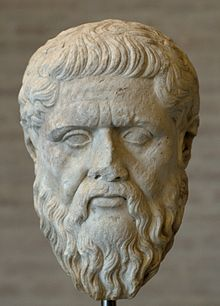
\includegraphics[width=0.3\textwidth]{Bilder/kap3/platon} 
	\caption{Platonportrait  \label{portraitPlaton}}
\end{figure}

\subsubsection{Kernthesen}

\paragraph{Wahrnehmung ist ungleich Wissen} 
Nach Platon ist die Wahrnehmung unserer fünf Sinne (sehen, hören, riechen, schmecken, fühlen) ungleich Wissen. Dies beweist er dadurch, dass Sinne Mängel aufweisen können. Ein Beispiel hierfür wären optische Täuschungen. Das Wissen wird laut ihm jedoch durch unsere Seele mit eigener Kraft  und denken erlangt. Wohingegen die Wahrnehmungen zwar von der Seele aufgenommen und verknüpft werden aber man durch sie keine Erkenntnis oder sicheres Wissen  erlangen kann.

\paragraph{Der Ursprung der Ideen} 
Hier unterscheidet Platon zwischen zwei Arten der Gleichheit.\newline
Zum Einen die Gleichheit der Dinge, hier entscheiden wir mit unseren Sinnen, ob zwei Gegenstände gleich sind oder nicht. Wir können so einen Apfel von einer Birne unterscheiden oder feststellen, dass ein Smartphone gleich einem weiteren Smarphone ist.\newline
Zum Anderen die Gleichheit an sich, diese findet in unserem Gehirn statt. Hier werden die Vorstellungen von Dingen miteinander verglichen.\newline
Das Beispiel mit den gleichen Smartphones zeigt dies sehr deutlich, dreht man eines um, ist die Gleichheit der Wahrnehmung anders. Die Gleichheit in unserer Vorstellung jedoch nicht. Daraus schließt Platon, dass die Vorstellung der Gleichheit gegenüber der Wahrnehmung der Gleichheit besser ist. Wenn man das feststellen kann, so Platon, muss man die Gleichheit an sich schon vorher gekannt haben. Und daraus schließt er, dass wir unsere Ideen schon vor der Geburt in uns haben, sie dann aber verlieren und sie im Laufe des Lebens zurück gewinnen und uns wieder daran erinnern müssen.

\paragraph{Ideenerkenntnis und Wissenschaft}
Platon veranschaulicht die Ideenerkenntnis und Wissenschaft an Gleichnissen. Diese werden in drei Stufen eingeteilt. Die Welt der sinnlichen Wahrnehmung (das Sichtbare), die Welt des Denkbaren (die Wissenschaft) und die Welt des Erkennbaren (die Vernunft). Nur in der letzten Stufe kann ein Mensch zur Erkenntnis kommen. Die letzte Welt beinhaltet das Reich der Ideen, dort liegt all das Wissen das wir vor der Geburt haben.
	
\subsubsection{Meinungsfindung}
Abschließend möchten wir diese Thesen verwenden, um eine mögliche Sichtweise Platons zu diesem Thema zu erörtern.

Zunächst erläutern wir hierzu die Aufgabe eines Chatbots mit künstlicher Intelligenz. Ein Chatbot wird häufig als Fragebeantworter im Kundenservice eingesetzt. Somit gibt er aus seiner künstlichen Welt Informationen weiter, die ein Mensch auf der anderen Seite des Monitors entgegennimmt.

Nehmen wir hierfür die These von Platon, dass Wahrnehmung ungleich Wissen ist. Da die Informationen nicht selbstständig durch eigene Kraft oder  nachdenken gewonnen wurden, sondern durch den Sehsinn, kann die Information kein Wissen sein. Ist aber nicht gerade das der Grund, warum mit dem Chatbot kommuniziert wird? Der unwissende Mensch möchte sich in diesem Szenario Wissen, das er nicht hat, aneignen. Anstatt selbst nachzudenken, geht er den bequemeren Weg, indem er den Chatbot fragt und wird womöglich, wie Platon beschrieb, von seinen Sinnen getäuscht.

Beziehen wir die These des Ursprungs der Ideen mit ein, wird die Sachlage schon schwieriger. Laut Platon haben wir die Ideen vor unserer Geburt in uns, verlieren sie bei der Geburt und müssen uns im  Laufe des Lebens wieder an sie erinnern. Das eine externe Hilfe hierbei behilflich sein darf oder überhaupt kann, sieht diese These nicht vor.

Um nun die Ideenerkenntnis und Wissenschaft einzubeziehen, müssen wir uns hier im klaren sein, auf welcher Stufe wir uns hier befinden. Ganz kritisch betrachtet liegt der Chatbot mit künstlicher Intelligenz in der Welt der sinnlichen Wahrnehmung, wie bereits in der ersten These feststellt werden kann. Geht man einen Schritt weiter kann behauptet werden, das der Chatbot in der Stufe der Wissenschaft anzusiedeln ist, da er aus mathematischen Funktionen besteht. Aber auch in dieser Stufe kann er den Menschen nicht zu Erkenntnis führen, dies geschieht erst in der Welt des Erkennbaren. Hierfür müsste man die Behauptung aufstellen, der Chatbot wäre in der Vernunft einzuordnen und wäre eventuell eine Informationsleitung aus dem Reich der Ideen um die Menschen daran zu erinnern, was sie vor der Geburt wussten.

\paragraph{Die Konklusion} ist nun, dass Platon wohl keinen Chatbot mit künstlicher Intelligenz als Wissensquelle nutzen würde. Vermutlich würde er die Informationen, die der Chatbot  weiter gibt gar nicht als Wissen ansehen. Wahrscheinlich würde er auch diesen Informationen, die von der Wahrnehmung aufgenommen werden, nicht vertrauen, denn diese täuschen oftmals. Er könnte auch den Weg, sich Wissen von etwas anderem anzueignen als seinen eigenen Gedanken, nicht unterstützen. Den sonst wäre es in seinen Augen kein Wissen und man würde als Mensch nie zur Erkenntnis gelangen. Was wiederum seinen Sinn des Lebens darstellt.     






